

\tikzset{every picture/.style={line width=0.75pt}} %set default line width to 0.75pt        

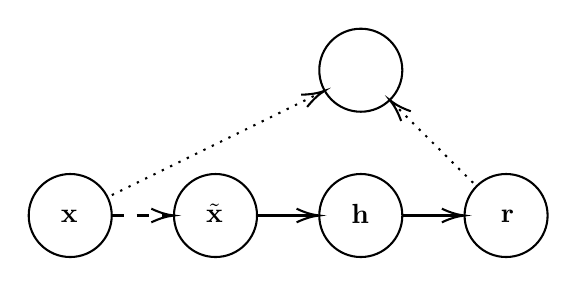
\begin{tikzpicture}[x=0.75pt,y=0.75pt,yscale=-1,xscale=1]
%uncomment if require: \path (0,300); %set diagram left start at 0, and has height of 300

%Straight Lines [id:da8399576495369319] 
\draw  [dash pattern={on 0.84pt off 2.51pt}]  (140,130) -- (260.72,70.8) ;
\draw [shift={(262.52,69.92)}, rotate = 513.88] [color={rgb, 255:red, 0; green, 0; blue, 0 }  ][line width=0.75]    (10.93,-3.29) .. controls (6.95,-1.4) and (3.31,-0.3) .. (0,0) .. controls (3.31,0.3) and (6.95,1.4) .. (10.93,3.29)   ;
%Shape: Boxed Line [id:dp10887462373342993] 
\draw  [dash pattern={on 0.84pt off 2.51pt}]  (349.96,130) -- (295.42,75.81) ;
\draw [shift={(294,74.4)}, rotate = 404.82] [color={rgb, 255:red, 0; green, 0; blue, 0 }  ][line width=0.75]    (10.93,-3.29) .. controls (6.95,-1.4) and (3.31,-0.3) .. (0,0) .. controls (3.31,0.3) and (6.95,1.4) .. (10.93,3.29)   ;
%Shape: Circle [id:dp5603710113663563] 
\draw   (260,130) .. controls (260,118.95) and (268.95,110) .. (280,110) .. controls (291.05,110) and (300,118.95) .. (300,130) .. controls (300,141.05) and (291.05,150) .. (280,150) .. controls (268.95,150) and (260,141.05) .. (260,130) -- cycle ;
%Shape: Circle [id:dp44224070274078864] 
\draw  [fill={rgb, 255:red, 255; green, 255; blue, 255 }  ,fill opacity=1 ] (190,130) .. controls (190,118.95) and (198.95,110) .. (210,110) .. controls (221.05,110) and (230,118.95) .. (230,130) .. controls (230,141.05) and (221.05,150) .. (210,150) .. controls (198.95,150) and (190,141.05) .. (190,130) -- cycle ;
%Shape: Circle [id:dp9930956365882191] 
\draw  [fill={rgb, 255:red, 255; green, 255; blue, 255 }  ,fill opacity=1 ] (330,130) .. controls (330,118.95) and (338.95,110) .. (350,110) .. controls (361.05,110) and (370,118.95) .. (370,130) .. controls (370,141.05) and (361.05,150) .. (350,150) .. controls (338.95,150) and (330,141.05) .. (330,130) -- cycle ;
%Shape: Circle [id:dp530216459507133] 
\draw   (260,60) .. controls (260,48.95) and (268.95,40) .. (280,40) .. controls (291.05,40) and (300,48.95) .. (300,60) .. controls (300,71.05) and (291.05,80) .. (280,80) .. controls (268.95,80) and (260,71.05) .. (260,60) -- cycle ;
%Straight Lines [id:da7671516825865974] 
\draw    (230,130) -- (258,130) ;
\draw [shift={(260,130)}, rotate = 180] [color={rgb, 255:red, 0; green, 0; blue, 0 }  ][line width=0.75]    (10.93,-3.29) .. controls (6.95,-1.4) and (3.31,-0.3) .. (0,0) .. controls (3.31,0.3) and (6.95,1.4) .. (10.93,3.29)   ;
%Straight Lines [id:da7943056265648183] 
\draw    (300,130) -- (328,130) ;
\draw [shift={(330,130)}, rotate = 180] [color={rgb, 255:red, 0; green, 0; blue, 0 }  ][line width=0.75]    (10.93,-3.29) .. controls (6.95,-1.4) and (3.31,-0.3) .. (0,0) .. controls (3.31,0.3) and (6.95,1.4) .. (10.93,3.29)   ;
%Shape: Circle [id:dp3989296686115751] 
\draw  [fill={rgb, 255:red, 255; green, 255; blue, 255 }  ,fill opacity=1 ] (120,130) .. controls (120,118.95) and (128.95,110) .. (140,110) .. controls (151.05,110) and (160,118.95) .. (160,130) .. controls (160,141.05) and (151.05,150) .. (140,150) .. controls (128.95,150) and (120,141.05) .. (120,130) -- cycle ;
%Straight Lines [id:da8399844169636741] 
\draw  [dash pattern={on 4.5pt off 4.5pt}]  (160,130) -- (188,130) ;
\draw [shift={(190,130)}, rotate = 180] [color={rgb, 255:red, 0; green, 0; blue, 0 }  ][line width=0.75]    (10.93,-3.29) .. controls (6.95,-1.4) and (3.31,-0.3) .. (0,0) .. controls (3.31,0.3) and (6.95,1.4) .. (10.93,3.29)   ;

% Text Node
\draw (134,126) node [anchor=north west][inner sep=0.75pt]    {$\mathbf{x}$};

% Text Node
\draw (204,123) node [anchor=north west][inner sep=0.75pt]    {$\tilde{\mathbf{x}}$};
% Text Node
\draw (274,123) node [anchor=north west][inner sep=0.75pt]    {$\mathbf{h}$};
% Text Node
\draw (346,126) node [anchor=north west][inner sep=0.75pt]    {$\mathbf{r}$};
% Text Node
\draw (273,52) node [anchor=north west][inner sep=0.75pt]    {$\Loss$};



\end{tikzpicture}